\documentclass[tikz,border=12pt]{standalone}
\usepackage[T1]{fontenc}
\usepackage{lmodern}
\usetikzlibrary{arrows.meta}
\tikzset{
  box/.style={draw,line width=1pt},
  w/.style={line width=.7pt,-{Latex[length=2.2mm]}},
  bus/.style={line width=1.8pt,-{Latex[length=3.2mm]}},
  dot/.style={circle,fill,inner sep=1.6pt},
  p/.style={font=\ttfamily\small,inner sep=1pt,text height=1.6ex,text depth=.45ex},
  t/.style={font=\sffamily\bfseries,inner sep=0pt}
}
\begin{document}
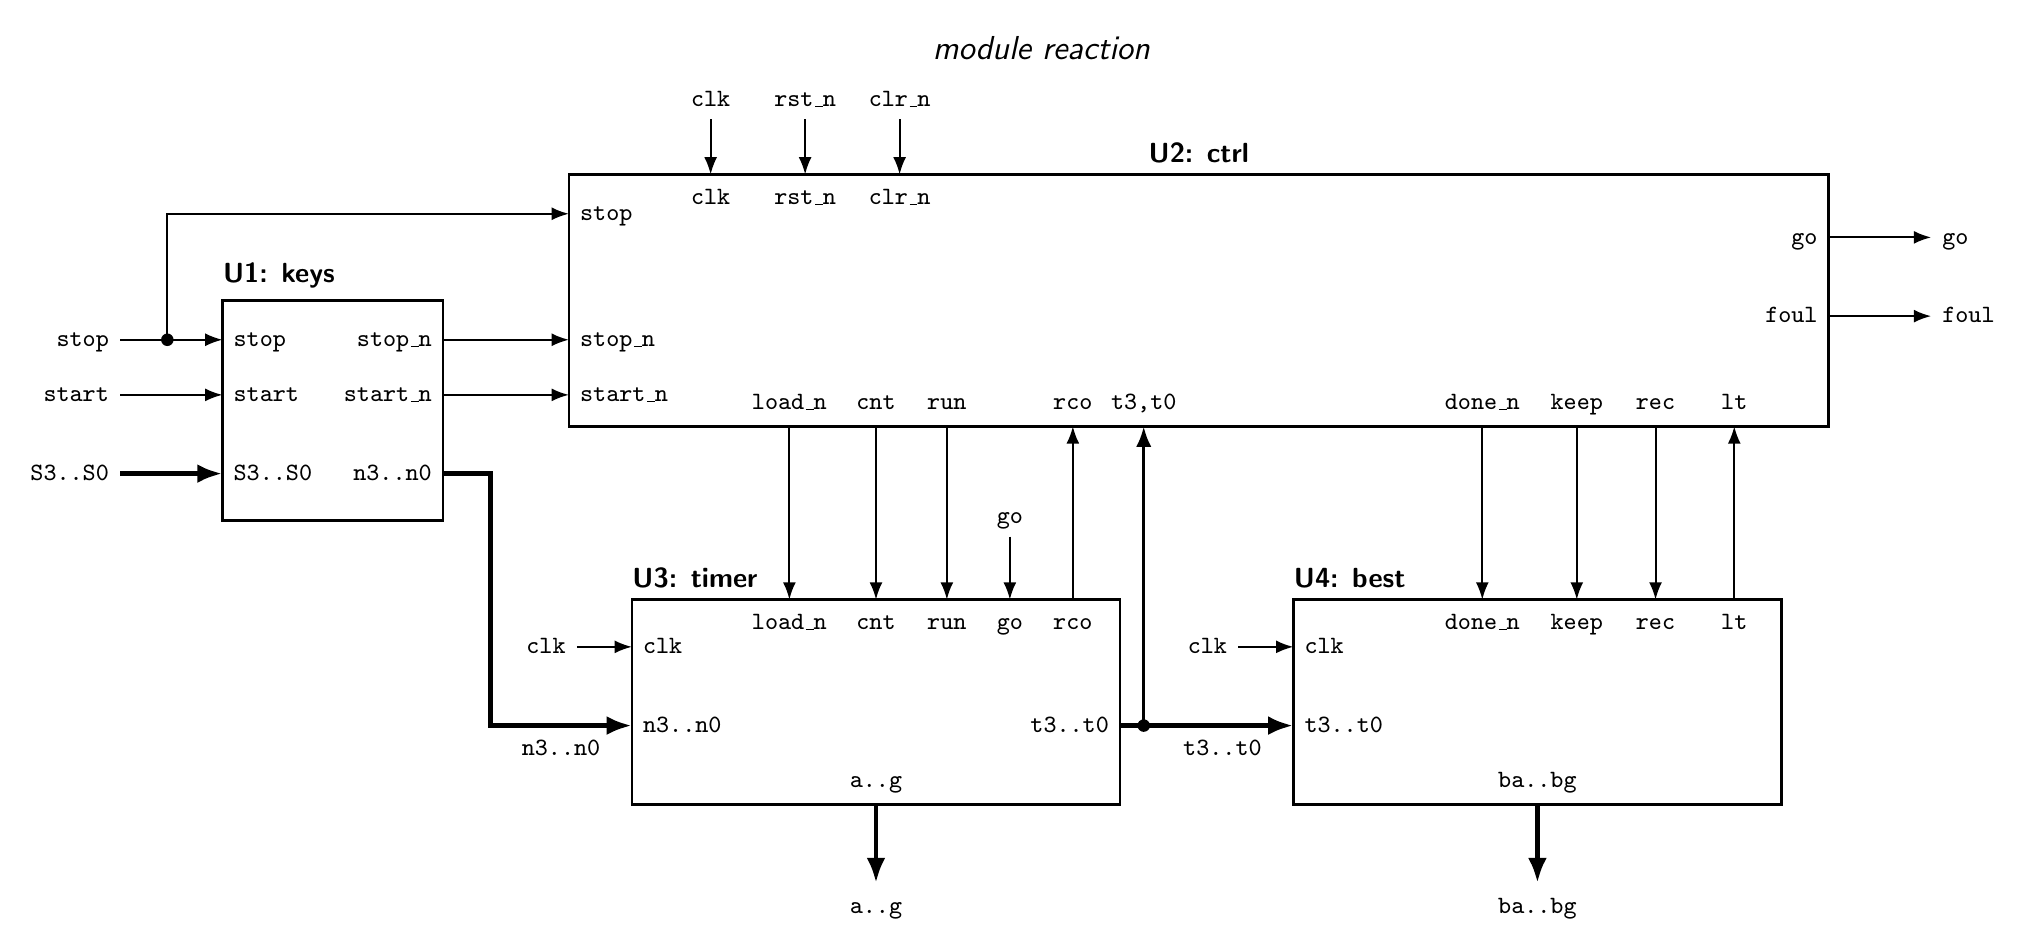
\begin{tikzpicture}
  \node[font=\sffamily\itshape\large] at (12.0,11.4) {module reaction};

  \draw[box] (1.6,5.4) rectangle (4.4,8.2);
  \draw[box] (6.0,6.6) rectangle (22.0,9.8);
  \draw[box] (6.8,1.8) rectangle (13.0,4.4);
  \draw[box] (15.2,1.8) rectangle (21.4,4.4);
  \node[t,anchor=south west] at (1.6,8.35) {U1: keys};
  \node[t,anchor=south] at (14.0,9.95) {U2: ctrl};
  \node[t,anchor=south west] at (6.8,4.55) {U3: timer};
  \node[t,anchor=south west] at (15.2,4.55) {U4: best};

  \draw[w] (0.3,7.7) -- (1.6,7.7);     \node[p,anchor=east] at (0.2,7.7) {stop};
  \draw[w] (0.3,7.0) -- (1.6,7.0);     \node[p,anchor=east] at (0.2,7.0) {start};
  \draw[bus] (0.3,6.0) -- (1.6,6.0);   \node[p,anchor=east] at (0.2,6.0) {S3..S0};
  \node[p,anchor=west] at (1.7,7.7) {stop};
  \node[p,anchor=west] at (1.7,7.0) {start};
  \node[p,anchor=west] at (1.7,6.0) {S3..S0};
  \node[p,anchor=east] at (4.3,7.7) {stop\_n};
  \node[p,anchor=east] at (4.3,7.0) {start\_n};
  \node[p,anchor=east] at (4.3,6.0) {n3..n0};

  \draw[w] (0.9,7.7) |- (6.0,9.3);
  \node[dot] at (0.9,7.7) {};
  \draw[w] (4.4,7.7) -- (6.0,7.7);
  \draw[w] (4.4,7.0) -- (6.0,7.0);
  \draw[bus] (4.4,6.0) -| (5.0,2.8) -- (6.8,2.8);
  \node[p,anchor=north] at (5.9,2.7) {n3..n0};

  \node[p,anchor=west] at (6.1,9.3) {stop};
  \node[p,anchor=west] at (6.1,7.7) {stop\_n};
  \node[p,anchor=west] at (6.1,7.0) {start\_n};
  \foreach \x/\n in {7.8/clk,9.0/rst\_n,10.2/clr\_n} {
    \draw[w] (\x,10.5) -- (\x,9.8);
    \node[p,anchor=south] at (\x,10.55) {\n};
    \node[p,anchor=north] at (\x,9.7) {\n};
  }
  \draw[w] (22.0,9.0) -- (23.3,9.0);   \node[p,anchor=west] at (23.4,9.0) {go};
  \draw[w] (22.0,8.0) -- (23.3,8.0);   \node[p,anchor=west] at (23.4,8.0) {foul};
  \node[p,anchor=east] at (21.9,9.0) {go};
  \node[p,anchor=east] at (21.9,8.0) {foul};
  \foreach \x/\n in {8.8/load\_n,9.9/cnt,10.8/run,12.4/rco,13.3/{t3,t0},17.6/done\_n,18.8/keep,19.8/rec,20.8/lt}
    \node[p,anchor=south] at (\x,6.7) {\n};

  \foreach \x in {8.8,9.9,10.8} \draw[w] (\x,6.6) -- (\x,4.4);
  \draw[w] (12.4,4.4) -- (12.4,6.6);
  \draw[w] (11.6,5.2) -- (11.6,4.4);   \node[p,anchor=south] at (11.6,5.25) {go};
  \draw[w] (6.1,3.8) -- (6.8,3.8);     \node[p,anchor=east] at (6.0,3.8) {clk};
  \node[p,anchor=west] at (6.9,3.8) {clk};
  \node[p,anchor=west] at (6.9,2.8) {n3..n0};
  \foreach \x/\n in {8.8/load\_n,9.9/cnt,10.8/run,11.6/go,12.4/rco}
    \node[p,anchor=north] at (\x,4.3) {\n};
  \node[p,anchor=east] at (12.9,2.8) {t3..t0};
  \node[p,anchor=south] at (9.9,1.9) {a..g};
  \draw[bus] (9.9,1.8) -- (9.9,0.8);   \node[p,anchor=north] at (9.9,0.7) {a..g};

  \draw[bus] (13.0,2.8) -- (15.2,2.8);
  \draw[line width=1.2pt,-{Latex[length=2.6mm]}] (13.3,2.8) -- (13.3,6.6);
  \node[dot] at (13.3,2.8) {};
  \node[p,anchor=north] at (14.3,2.7) {t3..t0};

  \draw[w] (14.5,3.8) -- (15.2,3.8);   \node[p,anchor=east] at (14.4,3.8) {clk};
  \node[p,anchor=west] at (15.3,3.8) {clk};
  \node[p,anchor=west] at (15.3,2.8) {t3..t0};
  \foreach \x/\n in {17.6/done\_n,18.8/keep,19.8/rec,20.8/lt}
    \node[p,anchor=north] at (\x,4.3) {\n};
  \foreach \x in {17.6,18.8,19.8} \draw[w] (\x,6.6) -- (\x,4.4);
  \draw[w] (20.8,4.4) -- (20.8,6.6);
  \node[p,anchor=south] at (18.3,1.9) {ba..bg};
  \draw[bus] (18.3,1.8) -- (18.3,0.8); \node[p,anchor=north] at (18.3,0.7) {ba..bg};
\end{tikzpicture}
\end{document}
